\chapter{Introduction}\label{ch:introduction}

First, this project is motivated by analyzing the need of robust facial expression recognition systems for various applications. Then already existing algorithms will be studied to choose one that is basic but effective in order to improve it. In our last part, we will formulate the problem.

 The next chapter is chapter~\ref{ch:ch2label}.

\section{Motivation}

A facial expression is a visible manifestation of the effective state, cognitive activity, intent, personality, and psychopathology of a person \cite{DON99}; facial expressions play a significant role in human dialogue and in human interaction. Indeed, facial expressions carry other information than speech and humans relay on that for their interaction. Facial expressions have a considerable effect on a listening interlocutor; the facial expression of a speaker accounts for about 55 percent of the effect, 38 percent of the latter is conveyed by voice intonation and 7 percent by the spoken words \cite{PAN00}.

Since antiquity, searchers have been interested in emotion and more particularly in emotion recognition. But one of the important works on facial expression analysis that has a direct relationship to the modern day science of automatic facial expression recognition was the work done by Charles Darwin [3]. In 1872, Darwin wrote a treatise that established the general principles of expression and the means of expressions in both humans and animals [4]. He also grouped various kinds of expressions into similar categories. This was the beginnings of facial expression recognition.

Now, with the emergence of the new technologies and the computers, searchers have put their interests on automatic facial expression recognition by computers. Because facial expressions are important in human interaction, this will add many possibilities in the domain of Human-Machine Interaction. Indeed with emotion recognition, the computers can be more responsive to the users' emotions and this way, interaction will not be as cold as the one we know. 

Another domain that is really interested in facial expression recognition is robotics. With the advances in robotics, now robots tend to mimic human emotion and to react as closely as humans as possible, especially for the humanoid robots. But because robots become a more and more important part in our lives, they need to understand and recognize human emotions.

But there is various other domains where emotion recognition can be used: Telecommunications, Behavioral Science, Video Games, Animations, Psychiatry, Automobile Safety, Affect sensitive music juke boxes and televisions, Educational Software, etc [3].

A lot of real time applications have already been created. For example, Bartlett et al. have successfully used their face expression recognition system to develop an animated character that mirrors the expressions of the user (called the CU Animate) [5]. They have also been successful in deployed the recognition system on Sony's Aibo Robot and ATR's RoboVie [5]. Another interesting application has been demonstrated by Anderson and McOwen, called the "EmotiChat" [6]. It is a chatroom where users can log in and start chatting. Their facial expression recognition system is connected to the chat and convert into emoticones the facial expression of the users. Because facial expression recognition system becomes more and more robust and more and more reliable, lot of innovative applications will turn out.

\subsection{Facial Expression Recognition system}

Facial Expression Recognition is a system that allows to recognize emotion on a human face in an automatic way. Facial Expression Recognition can be based on images or on videos; it can be real time or not. Most of the time, searchers use images of human faces and try to recognize the emotion. But this can also be done in real time by using video. While the person is having and expressing his emotions, the Facial Expression Recognition system is analyzing the video and detect in real time the emotion of the person.

In both cases, Facial Expression Recognition process is composed as follows:


\noindent 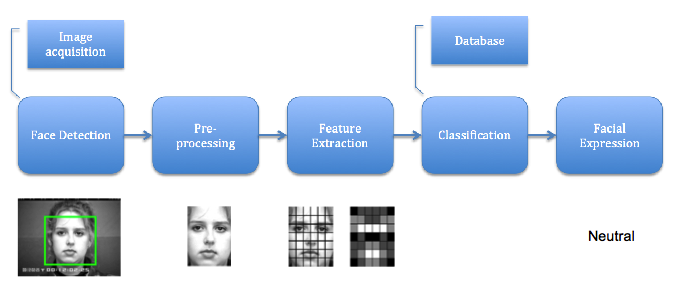
\includegraphics[scale=0.6]{figures/facial_expression_recognition_process}


You can also have examples in your document such as in example~\ref{ex:simple_example}.

\section{Existing systems}

Before developing our facial expression recognition project, it is important to know what already exist; the state of the art of facial expression recognition system. In this chapter, we will give an overview of the existing systems before we decide on a system for our project.

// ---------------------------- TEMPLATE EXAMPLES ---------------------------- 

\begin{example}{An Example of an Example}
  \label{ex:simple_example}
  Here is an example with some math
  \begin{equation}
    0 = \exp(i\pi)+1\ .
  \end{equation}
  You can adjust the colour and the line width in the {\tt macros.tex} file.
\end{example}

\section{How Does Sections, Subsections, and Subsections Look?}
Well, like this
\subsection{This is a Subsection}
and this
\subsubsection{This is a Subsubsection}
and this.

\paragraph{A Paragraph}
You can also use paragraph titles which look like this.

\subparagraph{A Subparagraph} Moreover, you can also use subparagraph titles which look like this\todo{Is it possible to add a subsubparagraph?}. They have a small indentation as opposed to the paragraph titles.

\todo[inline,color=green]{I think that a summary of this exciting chapter should be added.}
